% The shipped Realistix forecaster, drawn from the code.
%
% Every number here is read off `src/realistix/models/unet.py`,
% `src/realistix/models/uncertainty.py` and `tools/train_final.sh` rather than
% remembered: channel widths, grid sizes, parameter counts and the conditioning
% sites. Regenerate the counts with
%
%     PYTHONPATH=src python -c "from realistix.models import build_model, count_params; \
%         print(count_params(build_model(dict(width=96, cond='norm', film=True, \
%         mults='1,2,4', blocks=2))))"
%
% Build:  tectonic docs/model.tex          (or pdflatex; tikz only, no other packages)
%         pdftoppm -r 200 -png model.pdf docs/model
%
\documentclass[tikz,border=8pt]{standalone}
\usepackage{amsmath}
\usetikzlibrary{positioning,arrows.meta,fit,calc}

% ---------------------------------------------------------------- palette
\definecolor{cData}{HTML}{3C5C93}      % data and tensors
\definecolor{cConv}{HTML}{2F6B60}      % learned, shared across both domains
\definecolor{cCond}{HTML}{B5793A}      % per-domain parameters, folded at export
\definecolor{cHead}{HTML}{7E4E92}      % the interval head
\definecolor{cIdent}{HTML}{7A7A7A}     % exact, unlearned operations
\definecolor{cNote}{HTML}{5F5F5F}

\tikzset{
  box/.style={rounded corners=2pt, draw=#1, fill=#1!7, line width=0.7pt,
              inner sep=3pt, align=center, font=\sffamily\scriptsize,
              text=black},
  tensor/.style={box=cData, rounded corners=0pt},
  conv/.style={box=cConv},
  head/.style={box=cHead},
  ident/.style={box=cIdent, dashed},
  flow/.style={-{Stealth[length=4pt]}, line width=0.7pt, draw=cData!75!black},
  skipline/.style={flow, draw=cConv!75!black, dashed},
  note/.style={font=\sffamily\scriptsize, text=cNote, align=left},
  lbl/.style={font=\sffamily\tiny, text=cNote},
  title/.style={font=\sffamily\small\bfseries, align=left},
  % A conditioned site: the block carries its own per-domain affine.
  condmark/.style={circle, fill=cCond, draw=none, inner sep=0pt,
                   minimum size=3.4pt},
}
% Put the per-domain marker on a block's top-right corner.
\newcommand{\condat}[1]{\node[condmark] at ($(#1.north east)+(-2.2pt,-2.2pt)$) {};}

\begin{document}
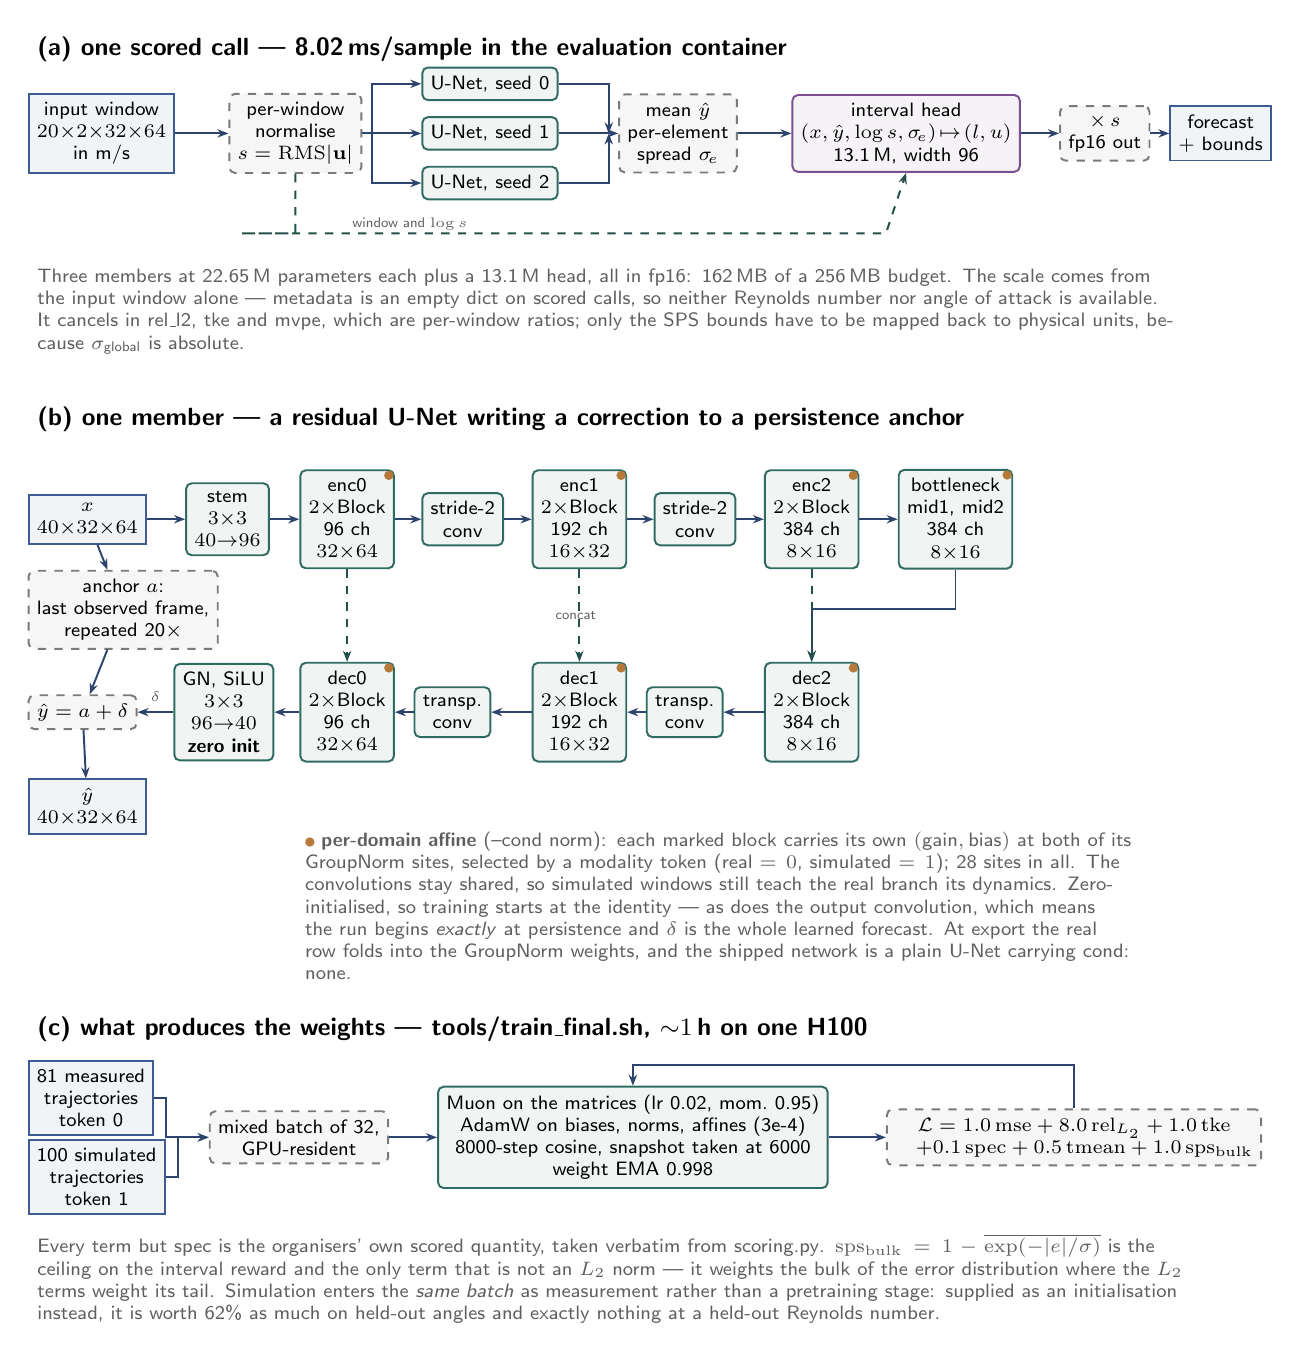
\begin{tikzpicture}[x=1cm, y=1cm]

% ==================================================================
% (a) the submission, end to end
% ==================================================================
\node[title, anchor=north west] at (0,0)
  {(a) one scored call --- 8.02\,ms/sample in the evaluation container};

\node[tensor, anchor=west]  (in)   at (0,-1.35)
  {input window\\$20{\times}2{\times}32{\times}64$\\in m/s};
\node[ident, anchor=west]   (norm) at (2.55,-1.35)
  {per-window\\normalise\\$s=\mathrm{RMS}|\mathbf u|$};
\node[conv, anchor=west, minimum width=13mm] (m1) at (5.0,-1.35) {U-Net, seed 1};
\node[conv, anchor=west, minimum width=13mm] (m0) at (5.0,-0.72) {U-Net, seed 0};
\node[conv, anchor=west, minimum width=13mm] (m2) at (5.0,-1.98) {U-Net, seed 2};
\node[ident, anchor=west]   (agg)  at (7.5,-1.35)
  {mean $\hat y$\\per-element\\spread $\sigma_{\!e}$};
\node[head, anchor=west]    (ih)   at (9.7,-1.35)
  {interval head\\$(x,\hat y,\log s,\sigma_{\!e})\!\mapsto\!(l,u)$\\13.1\,M, width 96};
\node[ident, anchor=west]   (den)  at (13.1,-1.35) {$\times\,s$\\fp16 out};
\node[tensor, anchor=west]  (out)  at (14.5,-1.35)
  {forecast\\ + bounds};

\draw[flow] (in) -- (norm);
\draw[flow] (norm.east) -- (m1.west);
\draw[flow] (norm.east) -- ++(0.12,0) |- (m0.west);
\draw[flow] (norm.east) -- ++(0.12,0) |- (m2.west);
\draw[flow] (m1.east) -- (agg.west);
\draw[flow] (m0.east) -| ($(agg.west)+(-0.12,0)$);
\draw[flow] (m2.east) -| ($(agg.west)+(-0.12,0)$);
\draw[flow] (agg) -- (ih);
\draw[flow] (ih) -- (den);
\draw[flow] (den) -- (out);
% the head reads the normalised window and log s directly as well
\draw[skipline] (norm.south) |- (2.7,-2.62) -- (10.9,-2.62) -- (ih.south);
\node[lbl, anchor=west] at (4.0,-2.5) {window and $\log s$};

\node[note, anchor=north west, text width=14.6cm] at (0,-2.95)
  {Three members at 22.65\,M parameters each plus a 13.1\,M head, all in fp16: 162\,MB of a
   256\,MB budget. The scale comes from the input window alone --- \textsf{metadata} is an
   empty dict on scored calls, so neither Reynolds number nor angle of attack is available.
   It cancels in \textsf{rel\_l2}, \textsf{tke} and \textsf{mvpe}, which are per-window
   ratios; only the SPS bounds have to be mapped back to physical units, because
   $\sigma_{\text{global}}$ is absolute.};

\begin{scope}[yshift=-0.75cm]
% ==================================================================
% (b) one member
% ==================================================================
\node[title, anchor=north west] at (0,-3.95)
  {(b) one member --- a residual U-Net writing a correction to a persistence anchor};

% the input, and the two things that come out of it
\node[tensor, anchor=west] (x)    at (0,-5.5)  {$x$\\$40{\times}32{\times}64$};
\node[ident,  anchor=west] (anch) at (0,-6.65) {anchor $a$:\\last observed frame,\\repeated 20$\times$};
\node[ident,  anchor=west] (sum)  at (0,-7.95) {$\hat y = a + \delta$};
\node[tensor, anchor=west] (yh)   at (0,-9.15) {$\hat y$\\$40{\times}32{\times}64$};

% encoder, left to right
\node[conv, anchor=west] (stem) at (2.0,-5.5) {stem\\$3{\times}3$\\$40{\to}96$};
\node[conv, anchor=west, minimum height=11mm] (e0) at (3.45,-5.5)
  {enc0\\$2\times$Block\\96 ch\\$32{\times}64$};
\node[conv, anchor=west] (p0) at (5.0,-5.5) {stride-2\\conv};
\node[conv, anchor=west, minimum height=11mm] (e1) at (6.4,-5.5)
  {enc1\\$2\times$Block\\192 ch\\$16{\times}32$};
\node[conv, anchor=west] (p1) at (7.95,-5.5) {stride-2\\conv};
\node[conv, anchor=west, minimum height=11mm] (e2) at (9.35,-5.5)
  {enc2\\$2\times$Block\\384 ch\\$8{\times}16$};
\node[conv, anchor=west, minimum height=11mm] (mid) at (11.05,-5.5)
  {bottleneck\\mid1, mid2\\384 ch\\$8{\times}16$};

\draw[flow] (x) -- (stem);
\draw[flow] (stem) -- (e0);
\draw[flow] (e0) -- (p0);
\draw[flow] (p0) -- (e1);
\draw[flow] (e1) -- (p1);
\draw[flow] (p1) -- (e2);
\draw[flow] (e2) -- (mid);

% decoder, right to left one row down
\node[conv, anchor=west, minimum height=11mm] (d2) at (9.35,-7.95)
  {dec2\\$2\times$Block\\384 ch\\$8{\times}16$};
\node[conv, anchor=west] (u1) at (7.85,-7.95) {transp.\\conv};
\node[conv, anchor=west, minimum height=11mm] (d1) at (6.4,-7.95)
  {dec1\\$2\times$Block\\192 ch\\$16{\times}32$};
\node[conv, anchor=west] (u0) at (4.9,-7.95) {transp.\\conv};
\node[conv, anchor=west, minimum height=11mm] (d0) at (3.45,-7.95)
  {dec0\\$2\times$Block\\96 ch\\$32{\times}64$};
\node[conv, anchor=west, minimum height=11mm] (outc) at (1.85,-7.95)
  {GN, SiLU\\$3{\times}3$\\$96{\to}40$\\\textbf{zero init}};

\draw[flow] (mid.south) -- ++(0,-0.5) -| (d2.north);
\draw[flow] (d2) -- (u1);
\draw[flow] (u1) -- (d1);
\draw[flow] (d1) -- (u0);
\draw[flow] (u0) -- (d0);
\draw[flow] (d0) -- (outc);

% concatenating skips
\draw[skipline] (e2.south) -- (d2.north);
\draw[skipline] (e1.south) -- (d1.north);
\draw[skipline] (e0.south) -- (d0.north);
\node[lbl, anchor=west] at (6.58,-6.72) {concat};

% the anchor path and the residual sum
\draw[flow] (x) -- (anch);
\draw[flow] (anch) -- (sum);
\draw[flow] (outc.west) -- node[lbl, above]{$\delta$} (sum.east);
\draw[flow] (sum) -- (yh);

% conditioning: mark the sites rather than draw seven arrows to them
\foreach \t in {e0,e1,e2,mid,d0,d1,d2}{\condat{\t}}
\node[note, anchor=north west, text width=10.6cm] at (3.4,-9.35)
  {\tikz\node[condmark]{}; \textbf{per-domain affine} (\textsf{--cond norm}): each marked
   block carries its own $(\text{gain},\text{bias})$ at both of its GroupNorm sites,
   selected by a modality token (real $=0$, simulated $=1$); 28 sites in all. The
   convolutions stay shared, so simulated windows still teach the real branch its
   dynamics. Zero-initialised, so training starts at the identity --- as does the output
   convolution, which means the run begins \emph{exactly} at persistence and $\delta$ is
   the whole learned forecast. At export the real row folds into the GroupNorm weights,
   and the shipped network is a plain U-Net carrying \textsf{cond: none}.};

% ==================================================================
% (c) training
% ==================================================================
\node[title, anchor=north west] at (0,-11.7)
  {(c) what produces the weights --- \textsf{tools/train\_final.sh}, ${\sim}1$\,h on one H100};

\node[tensor, anchor=west] (dr)   at (0,-12.85) {81 measured\\trajectories\\token 0};
\node[tensor, anchor=west] (dsim) at (0,-13.85) {100 simulated\\trajectories\\token 1};
\node[ident, anchor=west]  (mix)  at (2.3,-13.35) {mixed batch of 32,\\GPU-resident};
\node[conv, anchor=west]   (opt)  at (5.2,-13.35)
  {Muon on the matrices (lr 0.02, mom.\ 0.95)\\
   AdamW on biases, norms, affines (3e-4)\\
   8000-step cosine, snapshot taken at 6000\\
   weight EMA 0.998};
\node[ident, anchor=west]  (loss) at (10.9,-13.35)
  {$\mathcal L = 1.0\,\mathrm{mse} + 8.0\,\mathrm{rel}_{L_2}
     + 1.0\,\mathrm{tke}$\\
   $\quad + 0.1\,\mathrm{spec} + 0.5\,\mathrm{tmean}
     + 1.0\,\mathrm{sps_{bulk}}$};

\draw[flow] (dr.east)   -- ++(0.15,0) |- (mix.west);
\draw[flow] (dsim.east) -- ++(0.15,0) |- (mix.west);
\draw[flow] (mix) -- (opt);
\draw[flow] (opt) -- (loss);
\draw[flow] (loss.north) -- ++(0,0.55) -| (opt.north);

\node[note, anchor=north west, text width=14.6cm] at (0,-14.45)
  {Every term but \textsf{spec} is the organisers' own scored quantity, taken verbatim
   from \textsf{scoring.py}. $\mathrm{sps_{bulk}} = 1-\overline{\exp(-|e|/\sigma)}$ is
   the ceiling on the interval reward and the only term that is not an $L_2$ norm ---
   it weights the bulk of the error distribution where the $L_2$ terms weight its tail.
   Simulation enters the \emph{same batch} as measurement rather than a pretraining
   stage: supplied as an initialisation instead, it is worth 62\% as much on held-out
   angles and exactly nothing at a held-out Reynolds number.};

\end{scope}

\end{tikzpicture}
\end{document}
